%#!platex -kanji=utf8 hb.tex
\chapter{文書の構造}
% これはただのダミーテキスト.
% 文字コードを判定するための意味のない文字列.
% これくらい記述すれば大丈夫かな.
% Emacs のくせに生意気な.
% Emacs の分際で自動判別とか.
% Mac OS X のテキストエディッタの文字コード自動判別はうまくいかないぞ.

\section{章立て・見出し}
%文書に\KY{見出し} (\Z{sectioning}) と\K{目次} (\Z{contents}) がなければ,
%\Z{記事の検索}に時間がかかるのは容易に想像できるでしょう.そこで,
%文書の中には\K{階層的な見出し} (\Z{nested sections}) を作成します.
%\zindind{文書}{の概略}%
%またその文書の概略が存在すればその文書に何が書かれているのかがすぐ
%に分かるので,\K{概要} (\Z{abstract}) を付け足すのも効果的です.


\subsection{見出しの出力}\indindz{番号}{通し}%
%文書の中の一連の段落に何が書かれているのかを分かりやすくするために
%見出しを記述します.また見出しは同一ページに同じ名前のものが存在し
%ても良いように通し番号をつけて\Z{一意}的に管理します.

{\LaTeX}での見出しの定義は\tabref{headline}の通りです.%

\begin{table}[htpb]
 \begin{center}
  \caption{{\LaTeX}での見出しの定義}\tablab{headline}
  \newcommand{\midasiopt}{\opt{目次用の見出し}\param{見出し}}%
  \begin{tabular}{l|l}
   \TR
   \C{part}\midasiopt          & 部\\
   \C{chapter}\midasiopt       & 章${}^*$\\
   \C{section}\midasiopt       & 節\\
   \C{subsection}\midasiopt    & 項\pp{小節}\\
   \C{subsubsection}\midasiopt & 目\pp{小小節}\\
   \C{paragraph}\midasiopt     & 段落\\
   \C{subparagraph}\midasiopt  & 小段落\\
   \BR
  \end{tabular}
\\{\small${}^*$\Cls{article},\Cls{jarticle},\Cls{jsarticle}では定義されていません.}
 \end{center}
\end{table}

% \cmd{section}などの見出し命令を使って見出しを作成します.
%前後の空白の調節や改ページ,改行,書体の変更などはほぼ自動的に
%行われ,\KY{通し番号} (\Z{serial number})が付加されます.
%\zindind{目次}{用の見出し}%
%\indindz{見出し}{目次用の}%
%\qu{\opt{目次用の見出し}}という任意引数がありますが,
%これは見出しが非常に長いときに,それを短縮した文字列を目
%次に書き出すようにします.別に長いときだけではなく,
%見出しと目次の文字列を別にしたいときなどにも使えるでしょう.使い方
%は簡単です.見出しを階層構造的に書き記せば,{\LaTeX}は自動で階層ご
%とに番号付けをします.例としては次のような通し番号が振られます.

\begin{inonly}
\chapter{特殊相対性理論}
  \section{歴史的背景}
\chapter{一般相対性理論}
  \section{電気学との関連}
    \subsection{電気の次元数}
\end{inonly}
\begin{outonly}
{\Large \textbf{第1章 特殊相対性理論}}\\
{\large \textbf{1.1 歴史的背景}}\\
{\Large \textbf{第2章 一般相対性理論}}\\
{\large \textbf{2.1 電気学との関連}}\\
{\normalsize \textbf{2.1.1 電気の次元数}}
\end{outonly}%

\subsection{見出しの深さ}\zindind{見出し}{の深さ}%
\begin{table}[htpb]
%\begin{minipage}{.55\linewidth}
\caption{見出しの階層}\tablab{sectiondepth}
\begin{tabular}{lll}
\TR
\Th{見出し} & \Th{命令}     & \Th{深さ}${}^*$\\%$ 
\MR
部     & \Cmd{part}         & -1 \pp{0} \\
章     & \Cmd{chapter}      & 0  \pp{なし} \\
節     & \Cmd{section}      & 1   \\
小節   & \Cmd{subsection}   & 2   \\
小小節 & \Cmd{subsubsection}& 3   \\
段落   & \Cmd{paragraph}    & 4   \\
小段落 & \Cmd{subparagraph} & 4   \\ 
\BR
\multicolumn{3}{c}{${}^*$ 括弧内は\cls{(j)article}での深さ}
\end{tabular} 
%\end{minipage}
\end{table}

%\begin{minipage}{.44\linewidth}
\hskip1zw 文章の論理構造を整理するとき,一つの文書を{項目ごと}に分ける
事ができます.さらにその項目を小項目で分ける事もでき
るわけです.小項目があると文書の構造は{階層的に}なります.
項目が分かれている事を区別するために見出しを付けます.
見出しを\Z{目次}としてひとまとめに出力すると,読者は
目的の項目を探しやすくなります.\par
%\end{minipage}
%\end{table}
{\LaTeX}ではあらかじめ
部 (\Z{part}),
章 (\Z{chapter}),
節 (\Z{section}),
小節 (\Z{subsection}),
小小節 (\Z{subsubsection}),
段落 (\Z{paragraph}),
小段落 (\Z{subparagraph})
という七つの見出し用のコマンドを用意しています.
ただし\cls{(j)article}などで章は用意されていませんし,
クラスによって深さが若干違います. 




%\subsection{節見出しを中央揃えにする}

%%\centering
%\sty{jsclasses}の場合,
%\begin{intext}
%\newcommand{\section}{%
%  \if@slide\clearpage\fi
%  \@startsection{section}{1}{\z@}%
%  {\Cvs \@plus.5\Cdp \@minus.2\Cdp}% 前アキ
%  {.5\Cvs \@plus.3\Cdp}% 後アキ
%  {\normalfont\Large\headfont\raggedright}}
%\end{intext}
%を次のように変更します.
%% \makeatletter と \makeatother で括ります
%\begin{intext}
% \renewcommand{\section}{%
%  \if@slide\clearpage\fi
%  \@startsection{section}{1}{\z@}%
%  {\Cvs \@plus.5\Cdp \@minus.2\Cdp}% 前アキ
%  {.5\Cvs \@plus.3\Cdp}% 後アキ
%  {\normalfont\Large\headfont\centering}}
%\end{intext}


\subsection{あらかじめ定義されて見出しの名前を変更する}
\zindind{目次}{の見出しの変更}\zindind{見出し}{の変更}%
「目次」や「参考文献」などの見出しは \C{tableofcontents}命令や
\Env{thebibliography}環境によって出力されます.
この見出しの文字を変更するには次のようにします.
\begin{intext}
\renewcommand{\refname}{関連書籍}
\end{intext}

標準的な和文の文書クラスでは\tabref{midas:henko}
の見出しが定義されています.

\begin{table}[htbp]
\begin{center}\zindind{図}{目次}\zindind{表}{目次}%
\indindz{目次}{図}%
\indindz{目次}{表}%
\zindind{部}{の見出し}%
\zindind{章}{の見出し}%
\zindind{目次}{の見出し}%
\zindind{参考文献}{の見出し}%
\zindind{索引}{の見出し}%
\zindind{付録}{の見出し}%
\zindind{図}{の見出し}%
\zindind{表}{の見出し}%
\caption{定義済みの見出しの変更}\tablab{midas:henko}
 \begin{tabular}{lll}
 \TR
 \Th{命令}            & \Th{意味} & \Th{標準的な定義}\\
 \MR
 \C{prepartname}    & 部見出し番号の前の文字 & \Z{第}\\
 \C{postpartname}   & 部見出し番号の後の文字 & \W{部}\\
 \C{prechaptername} & 章見出し番号の前の文字 & \W{第}\\
 \C{postchaptername}& 章見出し番号の前の文字 & \W{章}\\
 \C{contentsname}   & 目次の見出しの     & \W{目次}\\
 \C{listfigurename} & 図目次の見出し   & \W{図目次}\\
 \C{listtablename}  & 表目次の見出し   & \W{表目次}\\
 \C{bibname}        & \env{thebibliography}環境の見出し& \W{参考文献}\\
 \C{figurename}     & 図見出し番号の前の文字& \W{図}\\
 \C{tablename}      & 表見出し番号の前の文字& \W{表}\\
 \C{appendixname}   & \env{appendix}環境での見出しの前の文字& \W{付録}\\
 \BR
 \end{tabular}
 \end{center}
\end{table}
\cmd{bibname}命令は\cls{jreport}や\cls{jbook}などでの定義で
\cls{(j)article}では \C{refname}となっています.
\hito{奥村}{晴彦}の\cls{jsclasses}では節見出し番号の前と後にも
文字列を表示できるようになっています.

\begin{intext}
\renewcommand{presectionname}{第}
\renewcommand{postsectionname}{節}
\end{intext}
上記のように \C{presectionname}や \C{postsectionname}を再定義します.

\section{目次}\seclab{目次}
\Z{目次}は見出しから読みたい箇所に移動するための\KY{見出し一覧}です.
これは数十ページ以上の文書に存在する事が望まれます.目次といっても
{\LaTeX}には次の三つの命令が用意されています.

\indindz{目次}{図}%
\indindz{目次}{表}%
\index{図目次}%
\index{表目次}%
\begin{usage}
\tableofcontents % 目次   (Contents)
\listoffigures   % 図目次 (List of Figures)
\listoftables    % 表目次 (List of Tables)
\end{usage}

目次を表示するためには,それぞれ出力したい場所に命令を書きます.
注意すべき事として,
\emph{目次を作成するためには最低2回のタイプセットを行います}.

%その理由を考えるために,以下のようなファイル\fl{mokuji.tex}を作ります.

\begin{inonly}
%#!platex  file.tex; dvipdfmx file; open file.pdf
\documentclass[a5j,report]{jsbook}
\setcounter{tocdepth}{2}% 次節で説明します.
\pagestyle{empty}
\begin{document}
 \tableofcontents
 \chapter{特殊相対性理論}
  \section{歴史的背景}
 \section{相対性と光速度の不変}
 \section{ローレンツ変換}
 \subsection{同時刻の相対性}
 \subsection{時間の遅れ}
 \subsection{ローレンツ収縮}
 \subsection{速度の合成}
 \subsection{光円錐と固有時}
 \section{相対論における「光速」}
 \chapter{一般相対性理論}
  \section{電気学との関連}
    \subsection{電気の次元数}
\end{document}
\end{inonly}

\begin{outonly}
\noindent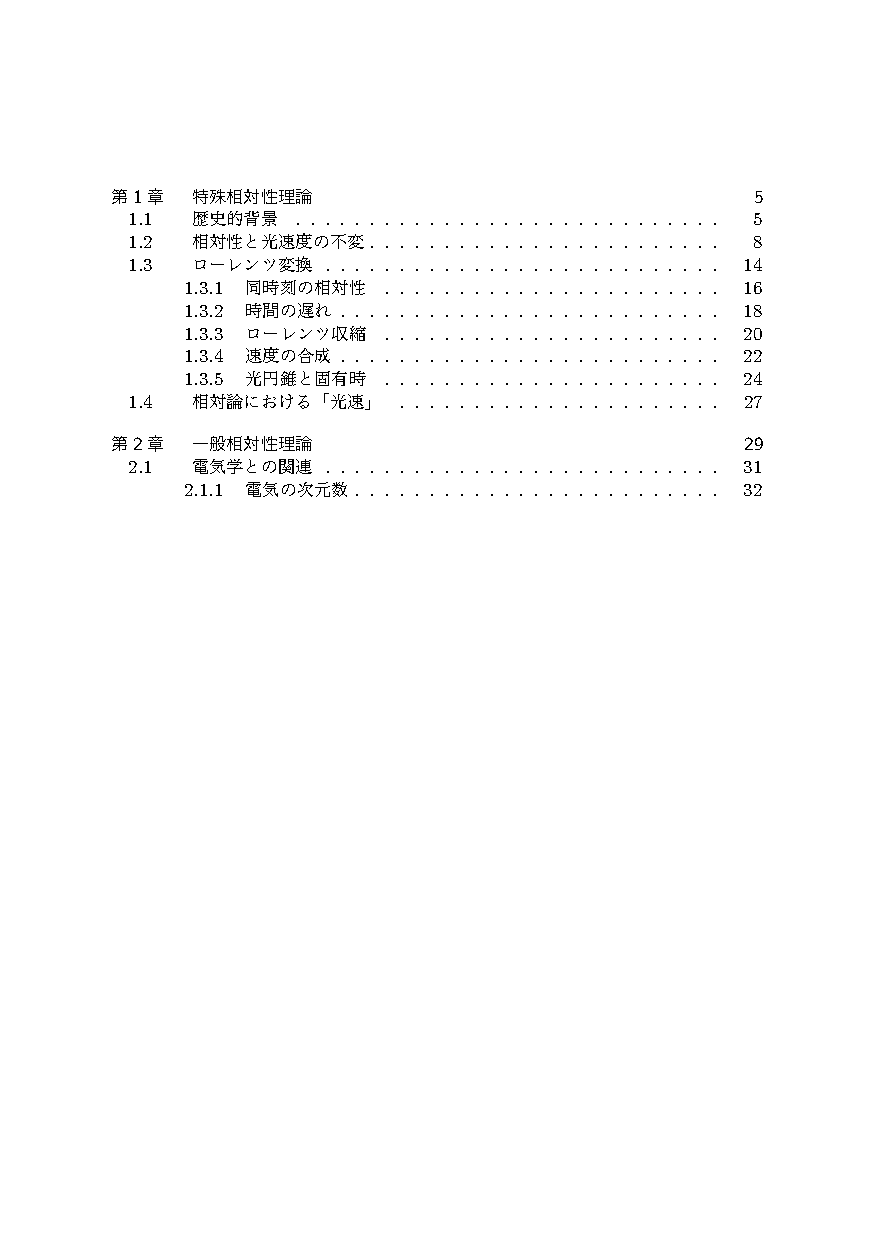
\includegraphics[width=\linewidth]{sample-toc}
\end{outonly}


\subsection{目次を出力する深さ}
\begin{usage}
\secounter{tocdepth}{$\<整数値>$} 
\end{usage}

\index{目次!tocdepth@\texttt{tocdepth}}%
\zindind{目次}{の深さ}%
%\index{カウンタ!tocdepth@\texttt{tocdepth}}%
目次をどの階層まで出力するかはカウンタ\Kount{tocdepth}の
値を\tabref{sectiondepth}に従って変更します.
\cls{jsbook}などで章\pp{\cmd{chapter}}まで出力したいならば
次のようにします.

\begin{intext}
\secounter{tocdepth}{0} 
\end{intext}

%\begin{InTeX}
%\secounter{tocdepth}{0}
%\end{InTeX}

\cls{(j)book}と\cls{(j)report}の標準は2,
\cls{(j)article}ならば3です.\cls{jsbook}は1になっています.

\secref{目次}では \cls{jsbook}クラスを用いています.
\cmd{subsection}までの見出しを目次に出力するために \kount{tocdepth}
を2に設定しています.\cls{jsbook}の標準では \cmd{section}までの見出し
しか出力されませんから,通常は次のように表示されます.
\begin{inonly}
\tableofcontents 
\end{inonly}
\begin{outonly}

\includegraphics[width=\linewidth]{sample-tocdepth}
\end{outonly}



\subsection{見出しの番号付けの深さ}
\begin{usage}
\setcounter{secnumdepth}{$\<整数値>$}
\end{usage}
\zindind{見出し}{の通し番号}%
\zindind{番号}{の深さ}%
\index{目次!secnumdepth@\texttt{secnumdepth}}%
\zindind{目次}{の番号付けの深さ}%
%\index{カウンタ!tocdepth@\texttt{secnumdepth}}%
見出しの通し番号はカウンタ\Kount{secnumdepth}によって
どの階層まで出力するかを決められます.\kount{secnumdepth}の
値は\tabref{sectiondepth}に従って変更します.
小節\pp{\cmd{subsection}}までに番号を付けるようにするには
次のようにします.これは目次側にも影響します.

\kount{secnumdepth}の値を変更すると,目次側も次のように変更されます.
\begin{inonly}
\setcounter{secnumdepth}{1}
\end{inonly}
\begin{outonly}
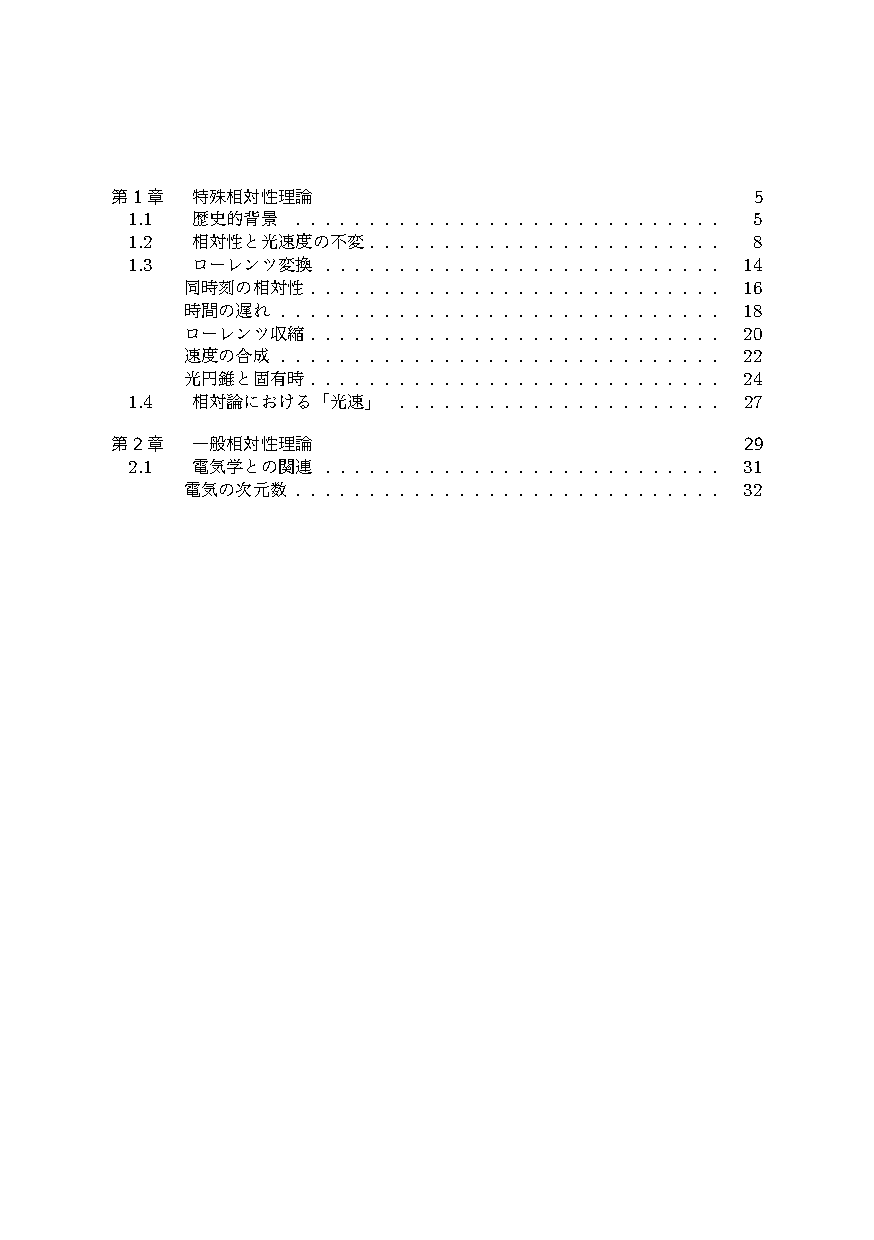
\includegraphics[width=\linewidth]{sample-secnumdepth1} 
\end{outonly}


\begin{inonly}
\setcounter{secnumdepth}{2}
\end{inonly}
\begin{outonly}
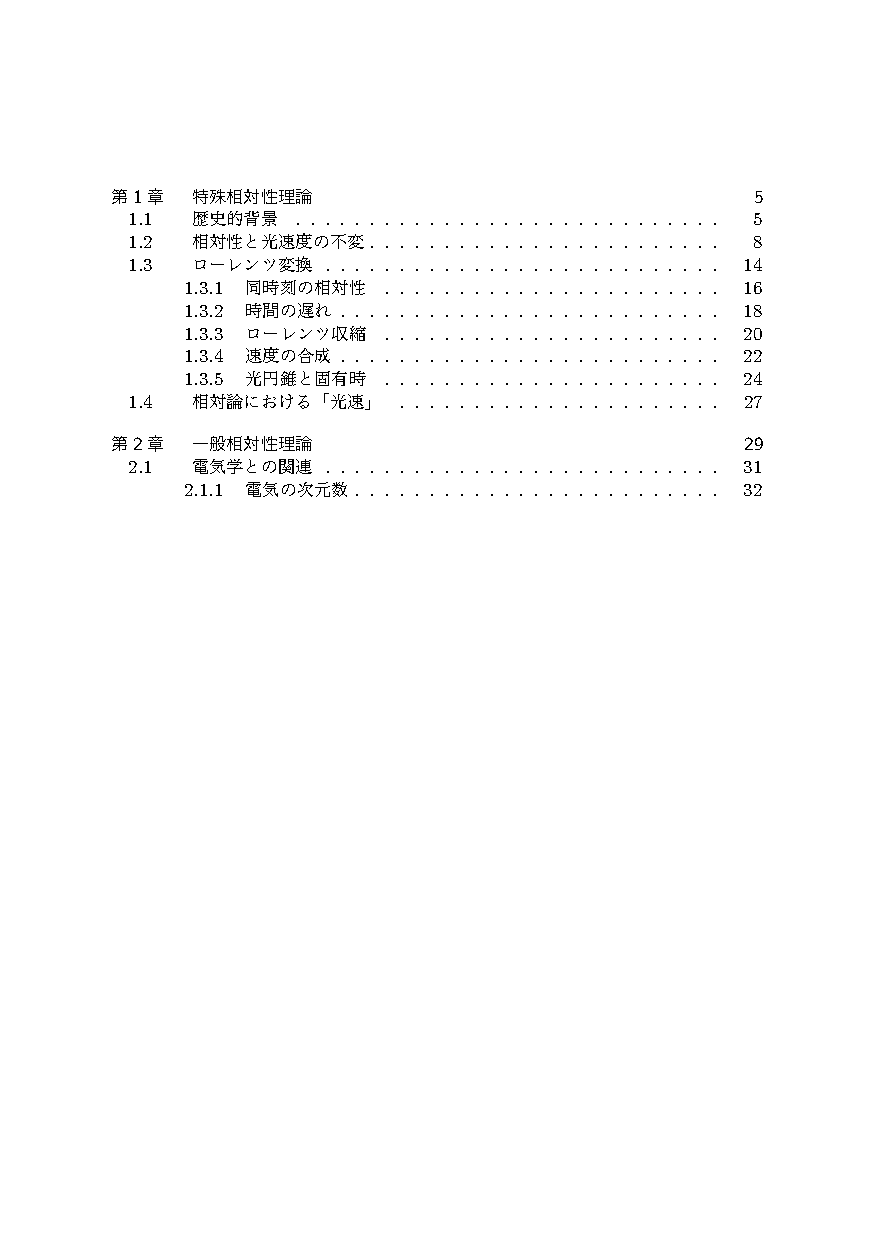
\includegraphics[width=\linewidth]{sample-secnumdepth2} 
\end{outonly}




\subsection{目次に独自に要素を追加する}
目次に出力される項目を制御したいときがあります.例え
ば見出し命令にアスタリスクをつけた場合\pp{\C{chapter*} など}は
通し番号が付かずに目次にも出力されません.
これを目次にも書き出すには次のようにします.
\begin{usage}
\addcontentsline{$\<拡張子>$}{$\<種類>$}{$\<要素>$}
\addtocontents{$\<拡張子>$}{$\<要素>$}
\end{usage}

例えば文書クラスに\cls{jreport}を使っていた場合に
\yo{謝辞}のような章を出力するときは次のように入力します.

\begin{intext}
\chapter*{謝辞}
ありがとう,本当にありがとう.
\end{intext}

しかしこれを目次にも追加するには \cmd{chapter*} の直後に記述します.

\begin{intext}
\chapter*{謝辞}\addcontentsline{toc}{chapter}{謝辞}
この文書を執筆する段階において,非常に多くの方々の
ご助言を頂いた.この場を借りて感謝の意を表す.
\end{intext}













\section{段落}
文章で段落をはじめようと思えば,まず\KY{字下げ} (\Z{indentation}) 
をします.%小学校の作文でも必ず作文用紙
%では次の段落に移るときは1文字開けたと思います.
この字下げの作業を{\LaTeX}は半自動で行います.使い方は
1行空けて入力すれば良いだけです.

\begin{inonly}
天皇は、日本国の象徴であり日本国民統合の象徴であつて、
この地位は、主権の存する日本国民の総意に基く。 

皇位は、世襲のものであつて、国会の議決した皇室典範の
定めるところにより、これを継承する。 

天皇の国事に関するすべての行為には、内閣の助言と承認
を必要とし、内閣が、その責任を負ふ。 
\end{inonly}
\begin{outonly}
 天皇は、日本国の象徴であり日本国民統合の象徴であつて、
この地位は、主権の存する日本国民の総意に基く。 

 皇位は、世襲のものであつて、国会の議決した皇室典範の
定めるところにより、これを継承する。 

 天皇の国事に関するすべての行為には、内閣の助言と承認
を必要とし、内閣が、その責任を負ふ。  
\end{outonly}

%\begin{OutText}
%\hskip1zw 天皇は、日本国の象徴であり日本国民統合の象徴であつて、
%この地位は、主権の存する日本国民の総意に基く。 \par
%\hskip1zw 皇位は、世襲のものであつて、国会の議決した皇室典範の
%定めるところにより、これを継承する。 \par
%\hskip1zw 天皇の国事に関するすべての行為には、内閣の助言と承認
%を必要とし、内閣が、その責任を負ふ。 
%\end{OutText}

このように自動的に字下げがなされます\footnote
   {『日本国憲法』 1947年5月3日\,施行の第1条から第3条までの引用.}.
明示的に \Cmd{par}命令で段落の開始を知らせる事ができます.

\CI{par}
\begin{usage}
\par % 明示的に段落のはじめを示す
\end{usage}

\begin{inonly}
天皇は、日本国の象徴であり日本国民統合の象徴であつて、
この地位は、主権の存する日本国民の総意に基く。\par
皇位は、世襲のものであつて、国会の議決した皇室典範の
定めるところにより、これを継承する。\par
天皇の国事に関するすべての行為には、内閣の助言と承認
を必要とし、内閣が、その責任を負ふ。\par
\end{inonly}
\begin{outonly}
 天皇は、日本国の象徴であり日本国民統合の象徴であつて、
この地位は、主権の存する日本国民の総意に基く。\par
 皇位は、世襲のものであつて、国会の議決した皇室典範の
定めるところにより、これを継承する。\par
 天皇の国事に関するすべての行為には、内閣の助言と承認
を必要とし、内閣が、その責任を負ふ。\par
\end{outonly}

\latexno{とワープロの違い}%
\indindz{改行}{原稿における}%
\indindz{改行}{出力結果における}%
\zindind{原稿}{中の改行}%
以上のように{\LaTeX}はワープロソフトとは違い,{原稿中の一つ
の改行が出力と対応していない}のがお分かりになるでしょう.
{\LaTeX}では{改行}すべき位置を自動で計算しているのです.



\subsection{行頭の字下げ}\seclab{indentfirst}
\zindind{字下げ}{の抑制}%
\zindind{行頭}{の字下げ}%
\indindz{字下げ}{行頭の}%

段落の開始には字下げをすべきなのですが,
何らかの理由により字下げを抑制したいときがあります.
字下げの有無に関しては \Cmd{indent} と \Cmd{noindent} 
命令が使えます.
\begin{usage}
\indent   % 行頭の字下げを誘発する
\noindent % 行頭の字下げを抑制する
\end{usage}
%\cls{jreport}などのクラスファイルではこのような命令を
%使っても行頭の字下げができないときがあります.
%その場合は\Sty{indentfirst}パッケージを読み込みます.
%\begin{inout}
%\usepackage{indentfirst}
%\noindent 私は\indent 大学生ですか
%ら,そうなります.\par
%\noindent そうなりました.
%\end{inout}

%\zindind{字下げ}{の幅の調節}%

\subsection{parindent}
\CI{parindent}%
\begin{usage}
\setlength{\parindent}{$\<字下げの幅>$}
\end{usage}
%\begin{Trick}
\indindz{幅}{字下げの}%
字下げの幅は \Cmd{parindent} という長さ変数で指定できます.
`\verb|\parindent = 3zw|'のようにすると約全角3文字分の字下げを段落の始め
で行う事ができます.
%\end{Trick}

\subsection{parskip}

%\begin{Prob}
行頭の字下げをせずに段落と段落に\Z{空き}を入れて段落の終わりと段落の始ま
りを示すという事を{\LaTeX}で行うためには,段落と段落の空きを調節す
る \C{parskip}という可変の長さ変数を調節します.

\begin{intext}
%\parindent = 0pt % 字下げ
\parskip = 10pt plus 0pt minus 0pt
\end{intext}

実際にこのような設定にすれば分かりますが,
ありとあらゆる部分に空きを挿入しますので,その出力結果を吟味してください.
%\end{Prob}

\subsection{段落の字下げ\zdash\Y{indent}}

\indindz{引用}{文の}%
\indindz{字下げ}{段落の}%
文を引用している場合はそれが\Z{引用}である事を明確に
するために,段落全体を字下げする習慣があります.
これには\Env{quote}環境や\env{quotation}環境が
使えます.ただしこの場合は自分で字下げ幅を
設定できません.%\env{quote}環境の中で使われている
%\Env{list}環境を自分でカスタマイズするとうまく行きます.
簡単に段落の字下げを調整するには\Sty{indent}パッケージの
\Env{indentation}環境を使います.

\begin{usage}
\begin{indentation}{$\<左側の字下げ幅>$}{$\<右側の字下げ幅>$}
 $\<文章要素>$
\end{indentation} 
\end{usage}

\env{indentation}環境の{一つ目}の必須引数には
{左側の}字下げ,{二つ目}には{右側の}字下げを指定します.
\begin{inout}
 ここは普通の文章領域です.不必要に字下げを調整するのは
 好ましいことではありません.
 \begin{indentation}{3zw}{3zw}
  左側の字下げは全角3文字分,右側の
  字下げも全角3文字分ありますか?
 \end{indentation}
 \begin{indentation}{0zw}{5zw}
  左側の字下げはなし,右側の字下げ
  は全角5文字分ありますか?
 \end{indentation}
 ここも普通の文章領域です.
\end{inout}

\subsection{ダブルスペース}\seclab{doublespace}
\Z{ダブルスペース}といって\KY{行送り}を倍にするという事を
迫られる場合があります.

これには \person{Geoffrey}{Tobin}による\Y{setspace}パッケージ
を使う事が考えられます\footnote{他にも \Y{doublespace}パッケージ
を使う方法や \Cmd{baselinestretch} 命令を再定義する方法もあります.}.
\begin{usage}
\singlespacing  % (通常通りの行送りに設定する)
\onehalfspacing % (通常の1.5倍の行送りにする)
\doublespacing  % (通常の2倍の行送りにする)
\end{usage}

\begin{usage}
\begin{spacing}{$\<行送りの割合>$}
 $\<文章要素>$
\end{spacing} 
\end{usage}

\va{数値}を指定して行送りを変更できる\Env{spacing}環境も用意されています.
%

\begin{inout}
\usepackage{setspace}
\singlespacing
ここは通常の\par 行間\par
\doublespacing
ここは通常の\par 2倍の行間\par
\begin{spacing}{.8}
ここは通常の\par 0.8倍の行間\par
\end{spacing}
\end{inout}











\section{引用}

\index{`@\verb+`+}\index{'@\verb+'+}\indindz{区切り}{文の}
文献から一文を引用する,段落を引用するという場面があると
思います.引用においては「いくつかの単語」,「文」,「段落」,
「複数の段落」の四つの引用形態があります.
\begin{description}
\indindz{引用}{単語の}\zindind{単語}{の引用}
 \item[単語の引用]
   欧文は\Z{シングルクオート} `~' を使い,
   和文は\Z{かぎ括弧} 「~」を使う.

\indindz{引用}{文の}\zindind{文}{の引用}
 \item[文の引用]  
   欧文は\Z{ダブルクオート} ``~'' を使い,
   和文は\Z{かぎ括弧} 「~」を使う.

\indindz{引用}{段落の}\zindind{段落}{の引用}
 \item[段落の引用]  
   \E{quote}環境を使い,別段落に組む.
   複数段落を記述しても,字下げが行なわれない.

\index{複数段落の引用}\indindz{引用}{複数段落の}
 \item[複数段落の引用]  
   \E{quotation}環境を使い,別段落に組む.
   各段落では字下げが行なわれる.
\zindind{引用}{の引用}
 \item[引用の引用]
   すでに引用している文をさらに引用するならば,
  欧文は`\,``~''\,'のようにし,
  和文は「~『~』~」とする.
\end{description}

シングルクオートも2種類あり左シングルクオート\pp{\str`}はキーボードの\keytop{Shift}を押しながら
\keytop{@}を押し,右シングルクオート\pp{\str'}は
\keytop{Shift}を押しながら\keytop{7}を押すと入力できると
思います.{\LaTeX}ではこれらを区別して記述します.
絶対に\key{Shift,2}を押して{ダブルクオート` \str" 'で%"
引用符を代用してはいけません}.

\indindz{引用}{文の}\zindind{文}{の引用}%
\K{文の引用}ではダブルクオートを使います.{Word}などで
ダブルクオートを挿入すれば自動的に\qq{一文}のように変換
されますが{\LaTeX}ではシングルクオートをうまく組み合わせ
て記述します.これは左シングルクオートを
二つと右シングルクオートを二つで括る事になります.
他に1文用の\Env{quote}環境や段落ごと引用するための
\Env{quotation}環境があります.

\begin{usage}
`単語の引用'
``文の引用''
\end{usage}

さらに段落ごと引用する場合は段落の左側を字下げして
出力します.場合によっては文字を小さくします.
一つの段落だけを引用する場合は\Env{quote}環境を,
複数の段落を引用するならば\Env{quotation}環境を使います.

\begin{usage}
\begin{quote}
 $\<単一の段落の引用テキスト>$
\end{quote} 
\end{usage}

\begin{usage}
\begin{quotation}
 $\<複数の段落の引用テキスト>$ 
\end{quotation} 
\end{usage}



%一般的に以下のような使い方になります.
\begin{inout}
`単語'の引用はシングルクオートで``文章
の一文''の引用は左シングルクオート二つ
と右シングルクオート二つです."ダブルク
オート"で引用符を表してはいけません.
\end{inout} 

\begin{inout}
 段落を引用する quote 環境については,
  \begin{quote}  
   行頭の字下げをする段落引用の quotation 環境が存在する.
  \end{quote}
 という説が知られている.
\end{inout}

和文の引用における\KY{引用符}は全角の\Z{かぎ括弧}\str{「」}を
使い,欧文の場合の引用符には{半角のクオート}\str{`'}を使います.
和文の引用の中の引用には\Z{二重括弧}を用います.和文の場合,
{括弧の中に句点を入れてはいけません}.
\begin{inout}
``FUN: Future University-Hakodate''
は恐らく`FUNNIST'との密接な関わりがあ
り,渡辺によると「未来らによると
『FUNNISTはFUNにある組織である』という
説がある」と考察している.
\end{inout}

%どちらか一方に統一するのが作成者側にも読者にも
%混乱は少ないでしょう.{\LaTeX}で引用というもの
%をもう少し効率良く行うには次のように定義します.

%\begin{intext}
%\newcommand{\qu}[1]{`#1'}%   単語の欧文引用 
%\newcommand{\qq}[1]{``#1''}% 1 文の欧文引用 
%\newcommand{\yo}[1]{「#1」}% 単語の和文引用 
%\newcommand{\yy}[1]{『#1』}% 1 文の和文引用 
%\end{intext}

%こうしておけば,後から引用符を統一できます.上記の \cmd{yo} と \cmd{yy}
%を次のように変更するだけで文章中の引用符を一括して
%変更できるわけです.

%\begin{intext}
%\newcommand{\yo}[1]{`#1'}% 単語の和文引用 
%\newcommand{\yy}[1]{``#1''}% 1 文の和文引用 
%\end{intext}

%\begin{InOut}
%それは渡辺らによれば\yo{デカルトの名言
%に\qu{I think, therefore I am.}があ
%る}という調査結果が存在する.
%\end{InOut}

%\subsection{書籍名や雑誌名の引用}
%
%\indindz{引用}{書籍名の}\indindz{引用}{雑誌名の}%
%\indindz{引用}{本の名前の}%
%\zindind{書籍名}{の引用}\zindind{雑誌名}{の引用}%
%\indindz{括弧}{引用のための}%
%\indindz{括弧}{書籍名のための}%
%\index{本の名前の引用}%
%\K{書籍名や雑誌名を引用}する場合はその名前を
%\K{イタリック体にします}.欧文の場合は \Cmd{emph} 命令を使います.
%和文の\K{書籍名を引用}する場合は\Z{二重かぎ括弧}『~』を,
%\K{雑誌名を引用}する場合はかぎ括弧「~」を使います.
%\begin{usage}
%\indindz{書籍}{和文の}%
%\indindz{雑誌}{和文の}%
%\C{emph}\pa{欧文の文献名}       \\
%『\va{書籍名}』\pp{和文の書籍}\\
%「\va{雑誌名}」\pp{和文の雑誌}
%\end{usage}
%以上のような方法を使って何か別の文書を示す場合はその文書名
%を強調表示します.
%\begin{InOut}
%渡辺が2004年に\emph{Natural}に投稿
%した論文「論文作成のいろは」は未来
%出版から『論文作成の手引き』に改題
%されて出版されている.
%\end{InOut}
%
%\begin{Trick}
%このような他の文書の引用には新たに欧文用の
%引用命令 \cmd{yousyo} や,和文用の \cmd{wasyo} などを
%作るとあとで統一したいときには便利でしょう.
%
%\begin{intext}
%\newcommand{\yousyo}[1]{\emph{#1}}%欧文
%\newcommand{\wasyo}[1]{『#1』}%和文
%\end{intext}
%
%\end{Trick}
%
%
%
%

\section{箇条書き} 
%\Z{箇条書き}には次の三つの環境を用いる事ができます.
\begin{itemize}
 \item 箇条書きの環境は\KY{入れ子}にできます.
 \item 入れ子にできる項目の深さは四つまでです.
 \item 入れ子のなった項目の先頭の記号は自動的に変更されます.
 \item \C{item} 命令を項目の先頭に記述します.
\end{itemize}

\subsection{記号付きの箇条書きを記述する}
\begin{usage}
\begin{itemize}
 \item $\<項目>{}_1$
 \item $\<項目>{}_2$
 …
\end{itemize} 
\end{usage}

\begin{inout}
\begin{itemize}
  \item ゼロ和ゲーム
  \item 非ゼロ和ゲーム
  \begin{itemize}
     \item 囚人のジレンマ・ゲーム
     \item MMORPG
    \end{itemize}
  \item 二人ゼロ和有限確定完全情報ゲーム
\end{itemize}
\end{inout}

%  項目の先頭に記号\pp{ラベル}が付く記号付き箇条書き環境.
%  環境の深さによって記号が\qu{$\bullet$,$-$,$*$,$\cdot$}
%  のように自動的に変わる.

\subsection{番号付きの箇条書きを記述する}
\begin{usage}
\begin{enumerate}
 \item $\<項目>{}_1$
 \item $\<項目>{}_2$
 …
\end{enumerate} 
\end{usage}

\begin{inout}
\begin{enumerate}
  \item  $R \leftarrow 1$ を実行する.
  \item  $N < 2 $ であれば $R$ を戻り値として返す.
  \item  $R \leftarrow R \times N$ を実行する.
  \item  $N \leftarrow N - 1$ を実行する.
  \item  ステップ2に戻る.
\end{enumerate} 
\end{inout}

%\indindz{番号}{箇条書きの}%
%  項目の先頭に通し番号が付く番号付き箇条書き環境.
%  深さによって通し番号が\qu{1,(a),i,A}
%  のように自動的に変わる.

\subsection{説明付きの箇条書きを記述する}
\begin{usage}
\begin{description}
 \item[$\<項目見出し>$] $\<項目>{}_1$
 \item[$\<項目見出し>$] $\<項目>{}_2$
 …
\end{description}  
\end{usage}

\begin{inout}
\begin{description}
  \item[日時] 2008年5月5日(月)13:00〜24:00
  \item[場所] 五稜郭公園(集合場所は第1駐車場です)
  \item[会費] 5,000円程度を予定しております
\end{description} 
\end{inout}

% 項目の前に説明を \cmd{item} の任意引数で指定する
%  説明付き箇条書き環境.

%\end{description}

%レポートや論文の場合はなるべく箇条書きは避けて,
%文章による記述が望ましいようです.理解のし
%やすさを考えれば箇条書きを使うべきでしょう.


%\subsection{番号付箇条書き環境の拡張\zdash\Y{enumerate}}\seclab{enumerate}
%
%番号付の箇条書き環境 \E{enumerate} の拡張を \Person{David}{Carlisle}が行な
%い,これを \Y{enumerate} パッケージとして用いる事ができます.
%\C{Alph}, \C{alph}, \C{Roman}, \C{roman}, \C{arabic} という命令の変わり
%に,次の文字 (トークン) によってカウンタとすべき\Z{修飾子}を決めます.
%
%\begin{usage}
%\begin{enumerate}[{$\<接頭辞>$}$\<修飾子>${$\<接尾辞>$}]
% \item[$\<項目見出し>$] $\<項目>{}_1$
% \item[$\<項目見出し>$] $\<項目>{}_2$
% $\vdots$
%\end{enumerate} 
%\end{usage}
%
%修飾子としたい文字は絶対に 波括弧 \{ \} でグルーピングしません.逆に
%修飾子と区別が付かない文字列 (Exmaple, A などなど) はグルーピングします.
%まずは,使用例を吟味してください.
%
%%\usepackage{okumacro,graphicx}
%\begin{inout}
%\usepackage{enumerate}
%\begin{enumerate}[{例題} 1]
%  \item\label{exe:a} 未来です.
%   \begin{enumerate}[{問題 \ref{exe:a}}-1]
%    \item これはどうか.
%    \item それはどうです.
%   \end{enumerate}
%  \item あれは云々.
%  \item これは云々.
%\end{enumerate}
%\end{inout}
%
%%\begin{Trick}
%\Z{丸数字}で番号付けをしたいとき等は \Y{okumacro} パッケージの \C{MARU} 命令
%を使います.このような特殊なケースは \Y{enumerate} パッケージを使わずに直
%接 \C{labelenumi} などのラベル部分を再定義した方が素直にできる場合もあ
%ります.
%
%\begin{intext}
%\begin{enumerate}
%\renewcommand\labelenumi{\MARU{\arabic{enumi}}}
%\item \TeX
%\item \LaTeX\,2.09
%\item \LaTeXe
%\item \LaTeX\,3
%\end{enumerate} 
%\end{intext}
%%\end{Trick}
%

\section{行揃え}
行揃えには三つの環境と三つの宣言型のコマンドを使う事ができます
\pp{\tabref{hss}}.
\begin{table}[htbp]%{l}{21zw}
\begin{center}
   \caption{揃えの命令と宣言}\tablab{hss}
  \begin{tabular}{*3l}
   \TR
   \Th{種類}     &\Th{環境} & \Th{宣言}\\   
   \MR
   左揃え   &\Env{flushleft}  & \Cmd{raggedright} \\
   中央揃え &\Env{center}     & \Cmd{centering} \\
   右揃え   &\Env{flushright} & \Cmd{raggedleft} \\   
   \BR
  \end{tabular}
\end{center}
\end{table}
環境型のコマンドは広い範囲に使い,宣言型のコマンドは
一つの要素や別の環境の中で使う事ができます.
\Z{中央揃え}には\Env{center}環境です.
1行もしくはそれ以上の文字列,表,図などを中央に寄せるこ%
\index{改行!きようそろえにおける@行揃えにおける\zdash}%
とが可能です.行頭や最終行に改行は入れません.
\Z{右揃え}には\Env{flushright}環境です.文字列を右寄せ
にします.\Z{左揃え}には\Env{flushleft}環境です.
字下げを行わずに左に寄せます.

\begin{inout}
ビジネス文書で大活躍するでしょう.
\begin{flushleft} 
段落の字下げを行わずに \\ 文字列を左に揃えます.
\end{flushleft}
\end{inout}

\begin{inout}
ビジネス文書で大活躍するでしょう.
\begin{center}
文章を\\ 中央揃えに \\ します.
\end{center}
\end{inout}

\begin{inout}
ビジネス文書で大活躍するでしょう.
\begin{flushright}
ビジネス文書で活躍中の\\ flushright
環境です.
\end{flushright}
\end{inout}

%さて,この三つの行揃えのコマンドを使って
%ありがちなビジネス文書の作成をしましょう.
この三つの行揃えのコマンドを使ってビジネス文書に良く見られる
書式を作成できます.\indindz{文書}{ビジネス}

\begin{inout}
\begin{flushright} 
   緊急連絡 \\    2004年3月31日
\end{flushright}
\begin{flushleft} 
   渡辺 徹殿
\end{flushleft}
\begin{flushright} 
   未来会社\\    人事課
\end{flushright}
\begin{center}
   人事異動のお知らせ
\end{center}
あなたは2004年度から檜山方面に配属されます.
\begin{flushright}  以上  \end{flushright}
\end{inout}

%このようにすると,以下のような出力となります.

%\begin{OutText}
%\begin{flushright} 緊急連絡 \\ 2004年3月31日\end{flushright}
%\begin{flushleft}  渡辺 徹殿                \end{flushleft}
%\begin{flushright} 未来会社\\ 人事課    \end{flushright}
%\begin{center}     人事異動のお知らせ       \end{center}
%あなたは2004年度から檜山方面に配属されます.
%\begin{flushright} 以上                     \end{flushright}
%\end{OutText}



\section{べた書き}
\index{書いたまま出力する}%
\index{入力通りの文字の出力}%
テキストをそのまま出力するときがあると思います.
例えば\Z{プログラムリスト}を載せたいときは\Z{特殊記号}
などが入り,そのままでは記述するのが困難です.
そのようなときは\KY{べた書き} (\Z{verbatim}) が可能です.
短い文字列の場合は \cmd{verb}命令を使います.

\begin{usage}
 \verb$\<区切り文字>$$\<そのまま出力した文字列>$$\<区切り文字>$
\end{usage}



\cmd{verb}命令や\env{verbatim}環境には
アスタリスクを付ける事ができます.さらに \cmd{verb}命令の
場合は\va{文字列}を括る区切り記号はアスタリスク`\str*'以外ならば
何でも良い事になっています.% \cmd{verb}命令に与えられた
%一つ目の区切りから二つ目の区切りに
\begin{inout}
\verb|2323 ^_^;|, \verb9|()|9.
\verb*|1 3 5|, \verb*9ok? ok?9.
\end{inout}

\subsection{複数行のベタ書きを記述する}
\begin{usage}
\begin{verbatim}
$\<ベタ書きにしたい文章要素>$	
\end{verbatim} 
\end{usage}


\begin{inout}
\verb|#include<stdio.h>| はプリプロセッサにより処理され…
\begin{verbatim}
int main (void){
   int foo = 0x7E;
   printf ("%c\n", foo); 
}
\end{verbatim}
\end{inout}


\subsection{複数行の空白が見えるベタ書きを記述する}
\begin{usage}
\begin{verbatim*}
$\<ベタ書きにしたい文章要素>$	
\end{verbatim*} 
\end{usage}
複数行になるときは\Env{verbatim}環境を使います.

\begin{verbatim*}
int main ( void ){
   printf ("Hello, World!\n"); 
}
\end{verbatim*}




\subsection{URLやemailを記述する}\seclab{url}
\begin{usage}
 \url{$\<http等から始まるURL>$}
\end{usage}


最近ではウェブ上への参照先を示すためにURLと呼ばれる
アドレスを書く場合があります.

これを{\LaTeX}でやろうと
思えば \cmd{verb}命令が使えると思うのですが\W{脚注}の中で使えないとか,
引数の中で使えないという事態に陥ります.このようなときは
\Person{Donald}{Arseneau}による\Sty{url}を使うと良いでしょう.
使い方は \cmd{verb}命令とほぼ同じで\qu{\texttt\%}や\qu{\texttt\#}
などの特殊記号に対して特別な対処をしなくともそのまま
記述できます.URLに対しては \C{url}を,
パスやファイルを示す場合は \C{path}を使います.e-mail
などを表記する場合は新規に \cmd{email}命令をを定義します.

\begin{intext}
\newcommand{\email}{\begingroup \urlstyle{rm}\Url}
\end{intext}

使われるフォントは \C{urlstyle}で指定します.
スラッシュやピリオドの位置などで自動的に改行されます.

\begin{inout}
\newcommand\email{\begingroup 
   \urlstyle{rm}\Url}
\newcommand\folder{\begingroup 
   \urlstyle{tt}\Url}
\url{ftp://www.any.com/dir/file.htm}
にアクセスしたら
\email{name@server.ac.jp}という
メールアドレスがあったので
\folder{/usr/local/bin/}
のファイルを消した.
\end{inout}




\section{複数のファイルに分ける}

 複数のファイルに分ける (include, input)

%\section{科学技術系文書の作成}





\section{注釈}

\subsection{脚注のパラメータ}

\begin{figure}[htbp]
 \begin{center}
  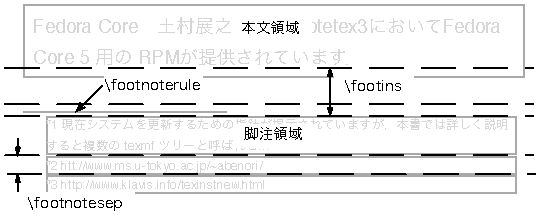
\includegraphics{footnotes}
 \end{center}
\end{figure}

%\subsection{脚注の記号を変更する}
%
%\begin{usage}
% \renewcommand\thefootnote{\fnsymbol{fotnote}}
%\end{usage}
%
%\begin{inout}
%\begin{minipage}{.9\linewidth}
%だめぽ
% \renewcommand\thefootnote{\fnsymbol{fotnote}}%%%%%HOGE
%\TeX\footnote{「テック」と発音する.}はDonald~E. Knuth,\LaTeX
%\footnote{「ラテック」と発音する.}はLeslie Lamportにより開発された.
%\end{minipage}
%\end{inout}

\subsection{注釈を一カ所にまとめる(後注)}

John Lavagnino氏による\Y{endnotes}を用いると,注釈を一カ所にまとめる事が
できます.

\begin{usage}
 \usepackage{endnotes}
 \endnote{$\<注釈内容>$}% \footnote と同様に記述する
 \theendnotes % 後注を出力したい場所に記述する
 \renewcommand{\notesname}{$\<後注見出し>$}
\end{usage}

\begin{inout}
\usepackage{endnotes}
hoge\endnote{a}
hoge\endnote{b}
\renewcommand{\notesname}{後注}
\theendnotes
\end{inout}

%\subsection{傍注}
%
%\zindind{注釈}{の役割}%
%\Z{注釈} (\Z{note}) とは文章の中で出てきた注意すべき語句を
%説明するために付けるものです.注釈は読者が読まなくても良い,
%本文とは関係のない情報を示すために使われます.{\LaTeX}では
%2種類の注釈を出力できます.
%\zindind{注釈}{の位置}%
%一つはページ下部に出力する\KY{脚注}\pp{\Cmd{footnote}},
%もう一つは注釈語の横に出力する\KY{傍注}%
%%\marginpar{このように\K{傍注}が出力されます}
%\pp{\Cmd{marginpar}}です.
%紙面の下端に表示される脚注には \Cmd{footnote} 命令を使います.
%\begin{usage}
%$\<用語>$\footnote{$\<注釈内容>$}
%\end{usage}
%
%レポート・論文の場合,{傍注を使わずに脚注のみを使うようにしてくださ
%い}.
%
%この命令を使用すると{\LaTeX}は組版時に自動的に \Cmd{footnote} で通し番号
%を付けます\footnote{このように注釈が文章の頁の下端に出力されます.}.
%脚注の出力は使用しているクラスファイルによって違うので確認してみると
%良いでしょう.
%\begin{inout}
%ラプラス変換やフーリエ変換\footnote
%{Fourier Translation}は通常理工系の
%大学ならば必修で\ldots と思われる.
%\end{inout}




\section{大規模な文書}


\subsection{原稿を複数のファイルに分ける}
\zindind{原稿}{の分割}%
大規模な文書になるとそれを一つのファイルにまとめるのは効
率が悪い場合があります.第3章は田中さんが編集し,第5章は斉
藤さんにお任せする,という状況では第3章と第5章の原稿は別
々に存在させたいものです.この場合は原稿を複数のファイル
に分けます.
\begin{usage}
\input{$\<ファイル名,\ldots>$}  % 
\include{$\<ファイル名,\ldots>$}% 改ページを伴う
\end{usage}

\cmd{include}命令はファイルを読み込むときに必ず新しいペ
ージから始めます.大規模な文書の章の区切りや節の区切りなど
で使用します.この命令で取り込むときはファイルを章ごとに
\pp{\cmd{chapter}ごと}に分ける事が考えられます.
\cmd{input}はそのままの意味で指定されたファイルを
そのまま親の{\LaTeX}のソースファイルに取り込みます.
取り込むファイルの拡張子が\exten{tex}ならば拡張子
を省略しても構いません.

\subsection{\protect\C{include}されている特定のファイルだけ読み込む}
\begin{usage}
\includeonly{$\<ファイル名>,\ldots$}
\end{usage}



例えば論文を作成する場合は次のように分割する事もできます.


\subsection{付録の追加}
\index{付録の追加}
文書の最後に付録としてプログラムリストを載せるとか,
本文とは直接的に関係のない資料を載せるときは \C{appendix}
命令を使うか,\Env{appendix}環境を
使うかの2通りの方法があります.\env{appendix}環境を
使う場合は付録の範囲を指定できます.
\begin{usage}
\begin{appendix}
\chapter{$\<付録中の見出し>_1$} 
$\<付録内容>_1$
\chapter{$\<付録中の見出し>_2$} 
$\<付録内容>_3$
$\vdots$
\end{appendix} 
\end{usage}
%あえて \cmd{appendix}命令を使う必要もないでしょう.
この命令を付けた後の文章は付録として扱われ,見出し
の番号付けが自動的に大文字のアルファベットに変更さ
れ,\qu{A}からカウントされるようになります.あとは
通常通り見出しの定義をして文章を記述するだけです.

\begin{usage}
\frontmatter % 前付の開始を宣言
\mainmatter  % 本文の開始を宣言
\backmatter  % 後付の開始を宣言
\end{usage}

\begin{center}
 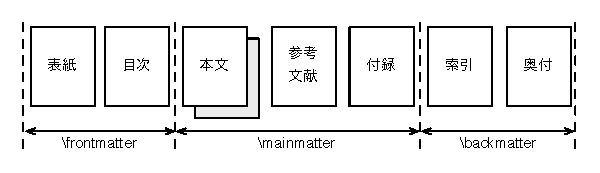
\includegraphics{matter}
\end{center}

\begin{intext}
%#!platex thesis.tex
\documentclass[dvipdfmx,papersize]{jsbook}% クラスファイル
\usepackage{amsmath,amssymb,verbatim,listings}% 必要なマクロ
\includeonly{2joron}% 特定の章だけを読み込む
\begin{document}
\maketitle
\tableofcontents
\listoffigures
\listoftables
\frontmatter%       前付
\include{0preface}% 前書き
\include{1thanx}%   謝辞
\mainmatter%        本文
%\doublespacing %     
\include{2joron}%   序論
\include{3honron}%  本論
\include{4keturon}% 結論
%\singlespacing %     
\begin{appendix}%   付録
\include{5code}%    付録: ソースコード
\end{appendix}%
\backmatter%        後付
\bibliographystyle{jplain}% 文献形式
\bibliography{ron}% 参考文献
\end{document}
\end{intext}
